\documentclass[a4paper,14pt]{extarticle}
\usepackage[english,russian]{babel}
\usepackage[cache=false]{minted}
\usepackage{fontspec}
\usepackage{indentfirst}
\usepackage{listings}
\usepackage{color}
\usepackage{caption}
\usepackage{amsmath}
\usepackage{hyperref}
\usepackage{graphicx}
\usepackage[%
    left=20mm,%
    right=10mm,%
    top=20mm,%
    bottom=20mm,%
]{geometry}%
\usepackage{titlesec}


\setmainfont{PT Astra Serif}

\hypersetup{
    colorlinks=true,
    linkcolor=black,
    filecolor=magenta,
    urlcolor=cyan,
    pdftitle={Лабораторная работа №4},
    pdfpagemode=FullScreen,
}

\newcommand{\hlink}[2]{\href{#1}{\color{blue}\underline{#2}}}
\graphicspath{ {./images/} }

\setmonofont[Scale=0.8]{JetBrains Mono}
\setminted{frame=lines, framesep=3mm, fontsize=\small}
\usemintedstyle{vs}

\titleformat{\section}
{\normalfont\bfseries}{}{0pt}{Упражнение \thesection.\;}

\titleformat{\subsection}
{\normalfont\bfseries}{}{0pt}{Задание \thesubsection.\;}

\numberwithin{figure}{section}

\begin{document}

\begin{titlepage}
    \vspace{0pt plus2fill}
    \noindent

    \vspace{0pt plus6fill}
    \begin{center}
        \textbf{\large{Санкт-Петербургский национальный исследовательский университет информационных
                технологий, механики и оптики}}

        \vspace{0pt plus2fill}
        \textbf{\Large{ЛАБОРАТОРНАЯ РАБОТА №7}}

        \vspace{0pt plus2fill}
        \textbf{\large{Создание иерархии классов}}
    \end{center}

    \vspace{0pt plus8fill}
    \begin{flushright}
        Студент: \\
        \textit{Швалов Даниил Андреевич}

        \textit{Факультет ИКТ}

        Группа: \textit{К32211}

        Преподаватель: \\
        \textit{Иванов Сергей Евгеньевич}
    \end{flushright}

    \vspace{0pt plus4fill}
    \begin{center}
        {Санкт-Петербург~--- 2023}
    \end{center}
\end{titlepage}

\section{Реализация наследования классов}

В проект был добавлен класс \texttt{Item}, который хранит в себе инвентарный номер \texttt{invNumber} и состояние объекта \texttt{taken}, а также имеет соответствующие методы для их изменения. Кроме того, в класс \texttt{Item} был добавлен метод, выводящий информацию на экран об единице хранения:

\inputminted{csharp}{../MyClass/MyClass/Item.cs}

В класс \texttt{Book} добавлено наследование от класса \texttt{Item}, а также определен метод \texttt{TakeItem}:

\inputminted{csharp}{../MyClass/MyClass/Book.cs}

В класс \texttt{Program} был добавлен код, проверяющий работу программы:

\inputminted{csharp}{../MyClass/MyClass/Program.cs}

На рис. \ref{fig:task-1} представлен пример работы программы.

\begin{figure}[H]
    \centering
    
\includegraphics[width=0.5\textwidth]{images/task-1.png}
    \caption{Пример работы программы}
    \label{fig:task-1}
\end{figure}

\section{Использование конструкторов}

В класс \texttt{Item} было добавлено два конструктора: один с аргументами, а второй по умолчанию:

\inputminted{csharp}{../MyClass1/MyClass/Item.cs}

В класс \texttt{Book} был добавлен конструктор со ссылкой на конструктор базового класса. В метод \texttt{Show} был добавлен вызов метода базового класса:

\inputminted{csharp}{../MyClass1/MyClass/Book.cs}

В проект был добавлен класс \texttt{Magazine}, хранящий в себе название тома \texttt{volume}, его номер \texttt{number}, название журнала \texttt{title} и год выпуска \texttt{year}. В класс \texttt{Magazine} был добавлен конструктор по умолчанию, а также конструктор, принимающий данные о журнале. Кроме того, был добавлен метод \texttt{Show}, отображающий информацию о журнале:

\inputminted{csharp}{../MyClass1/MyClass/Magazine.cs}

В класс \texttt{Program} был добавлен код, проверяющий работу программы:

\inputminted{csharp}{../MyClass1/MyClass/Program.cs}

На рис. \ref{fig:task-2} представлен пример работы программы.

\begin{figure}[H]
    \centering
    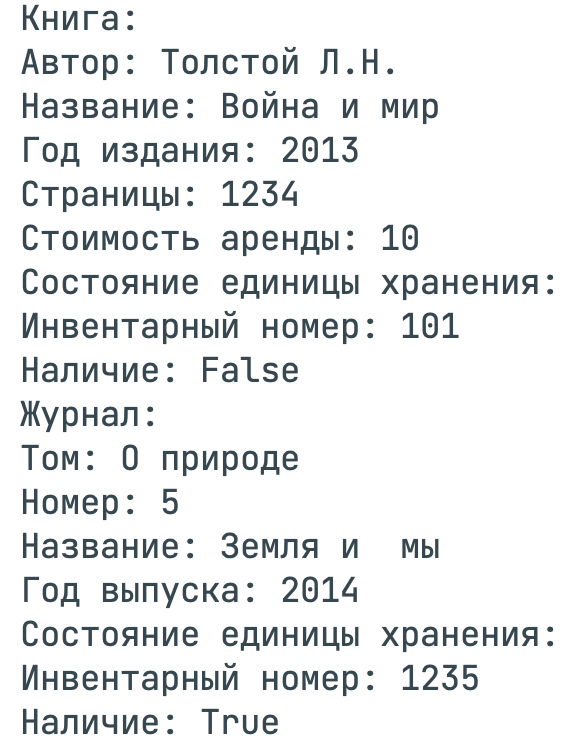
\includegraphics[width=0.4\textwidth]{images/task-2.png}
    \caption{Пример работы программы}
    \label{fig:task-2}
\end{figure}

\section{Переопределение методов}

В классе \texttt{Item} метод \texttt{Return} был помечен как виртуальный:

\inputminted{csharp}{../MyClass2/MyClass/Item.cs}

В класс \texttt{Book} было добавлено новое поле \texttt{returnSrok}, а также метод \texttt{ReturnSrok}, устанавливающий, что книга сдана в срок. Кроме того, был переопределен метод \texttt{Return}:

\inputminted{csharp}{../MyClass2/MyClass/Book.cs}

В классе \texttt{Magazine} тоже был переопределен метод \texttt{Return}:

\inputminted{csharp}{../MyClass2/MyClass/Magazine.cs}

В класс \texttt{Program} был добавлен код, проверяющий работу программы:

\inputminted{csharp}{../MyClass2/MyClass/Program.cs}

На рис. \ref{fig:task-3} представлен пример работы программы.

\begin{figure}[H]
    \centering
    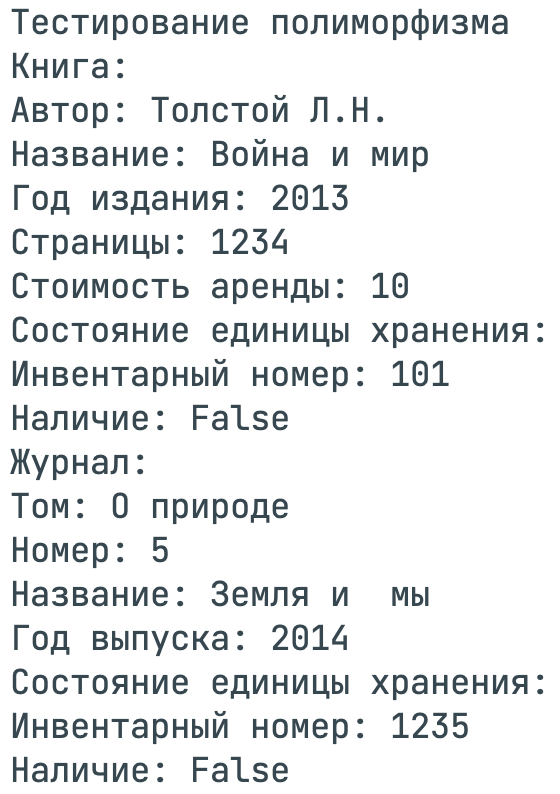
\includegraphics[width=0.4\textwidth]{images/task-3.png}
    \caption{Пример работы программы}
    \label{fig:task-3}
\end{figure}

\section{Применение абстрактного класса и абстрактных методов}

Класс \texttt{Item}, а также его метод \texttt{Return} был помечен как абстрактный:

\inputminted{csharp}{../MyClass3/MyClass/Item.cs}

Остальные классы остались без изменения:

\inputminted{csharp}{../MyClass3/MyClass/Book.cs}

\inputminted{csharp}{../MyClass3/MyClass/Magazine.cs}

В класс \texttt{Program} был добавлен код, проверяющий работу программы:

\inputminted{csharp}{../MyClass3/MyClass/Program.cs}

На рис. \ref{fig:task-4} представлен пример работы программы.

\begin{figure}[H]
    \centering
    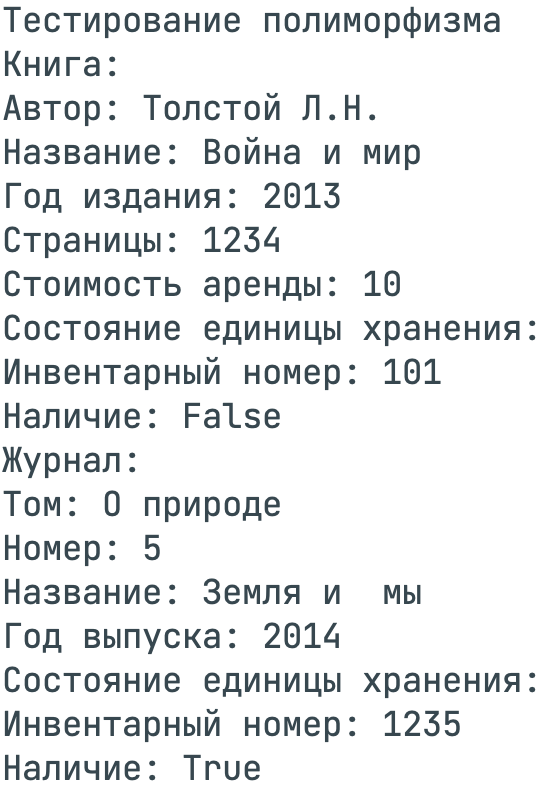
\includegraphics[width=0.4\textwidth]{images/task-4.png}
    \caption{Пример работы программы}
    \label{fig:task-4}
\end{figure}

\section{Реализации модели включения}

В проект был добавлен класс \texttt{Point}, содержащий координаты \texttt{x} и \texttt{y}. Также в класс был добавлен конструктор, принимающий эти координаты. Кроме того, в класс были добавлены методы \texttt{Show} для отображения информации о точке, \texttt{Dlina} для вычисления расстояния между двумя точками и \texttt{ToString} для отображения объекта:

\inputminted{csharp}{../MyClassLine/Point.cs}

В проект был добавлен класс \texttt{Line}, содержащий начальную \texttt{pStart} и конечную \texttt{pEnd} точки. Также в класс был добавлен конструктор, принимающий начальную и конечную точку. Кроме того, были добавлены методы \texttt{Show} для отображения информации об отрезке, а также \texttt{DlinL} для вычисления длины отрезка:

\inputminted{csharp}{../MyClassLine/Line.cs}

В класс \texttt{Program} был добавлен код, проверяющий работу программы:

\inputminted{csharp}{../MyClassLine/Program.cs}

На рис. \ref{fig:task-5} представлен пример работы программы.

\begin{figure}[H]
    \centering
    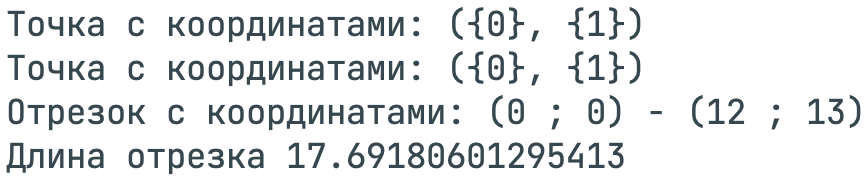
\includegraphics[width=0.4\textwidth]{images/task-5.png}
    \caption{Пример работы программы}
    \label{fig:task-5}
\end{figure}

\section{Реализация отношения ассоциации между классами}

В проект был добавлен класс \texttt{IgralnayaKost}, хранящий генератор псевдослучайных чисел \texttt{r}. Для него был создан конструктор по умолчанию, создающий генератор псевдослучайных чисел. Также в класс был добавлен метод \texttt{random}, возвращающий случайное число в диапазоне от 1 до 6:

\inputminted{csharp}{../Igra/IgralnayaKost.cs}

В проект был добавлен класс \texttt{Gamer}, хранящий имя \texttt{name} и игральную кость \texttt{seans}. Для него был реализован конструктор, принимающий имя игрока. Кроме того, были добавлены методы \texttt{SeansGame} для броска кости и \texttt{ToString} для отображения объекта:

\inputminted{csharp}{../Igra/Gamer.cs}

В класс \texttt{Program} был добавлен код, проверяющий работу программы:

\inputminted{csharp}{../Igra/Program.cs}

На рис. \ref{fig:task-6} представлен пример работы программы.

\begin{figure}[H]
    \centering
    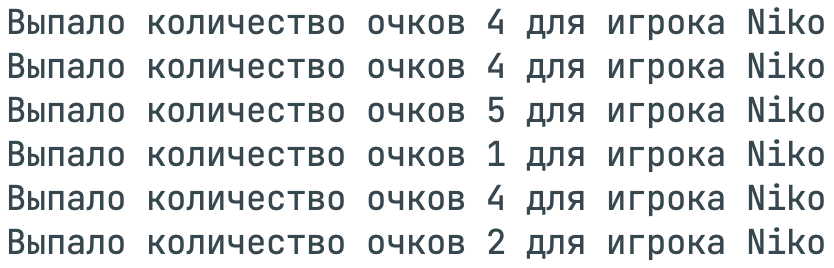
\includegraphics[width=0.6\textwidth]{images/task-6.png}
    \caption{Пример работы программы}
    \label{fig:task-6}
\end{figure}

\section{Реализация прогрессии}

В проект был добавлен абстрактный класс \texttt{Progression}, в который был добавлен абстрактный метод \texttt{GetElement}, возвращающий k-ый элемент прогрессии:

\inputminted{csharp}{../Progression/Progression.cs}

В проект был добавлен класс \texttt{ArithmeticProgression}, реализующий арифметическую прогрессию. Конструктор этого класса принимает первый член прогрессии \texttt{firstMember} и разность прогрессии \texttt{difference}:

\inputminted{csharp}{../Progression/ArithmeticProgression.cs}

В проект также был добавлен класс \texttt{GeometricProgression}, представляющий геометрическую прогрессию. Конструктор этого класса принимает первый член прогрессии \texttt{firstMember} и знаменатель прогрессии \texttt{denominator}:

\inputminted{csharp}{../Progression/GeometricProgression.cs}

В класс \texttt{Program} был добавлен код, проверяющий работу программы:

\inputminted{csharp}{../Progression/Program.cs}

На рис. \ref{fig:task-7} представлен пример работы программы.

\begin{figure}[H]
    \centering
    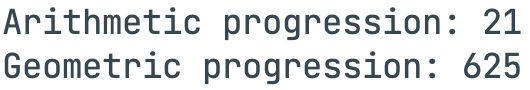
\includegraphics[width=0.5\textwidth]{images/task-7.png}
    \caption{Пример работы программы}
    \label{fig:task-7}
\end{figure}

\end{document}
